\documentclass[12pt,a4paper,titlepage,twoside]{report}
\usepackage[T1]{fontenc}
\usepackage[english, spanish,es-tabla]{babel}
\usepackage[utf8]{inputenc}
\usepackage[style=spanish]{csquotes}

%Latin modern font
\usepackage{lmodern}
\usepackage{tabularx}
%\usepackage[backend=bibtex]{biblatex}
%\bibliography{bibliografia.bib} % or

\usepackage{hyperref}
\usepackage{bookmark}
\usepackage[numbers]{natbib}

\usepackage{graphicx}
% Con esta opción no cargo las imágenes sólo sus espacios
%\usepackage[draft]{graphicx}
\usepackage{wrapfig} %Las imágenes quedan rodeadas de texto

%Interlineado
\usepackage{setspace}

% Parámetro para poder usar los colorines
\usepackage[pdftex,usenames,dvipsnames,table]{xcolor}
%Paquete para justificar el texto
\usepackage{ragged2e} 
\usepackage{notoccite}

% Penalizo la finalización o el inicio de la página con 
% lineas huerfanas
%\clubpenalty=10000
%\widowpenalty=10000

\usepackage[nottoc,numbib]{tocbibind}
\usepackage[toc,page]{appendix}

%Fancy chapter
\usepackage{titlesec, blindtext, color}
\definecolor{gray75}{gray}{0.75}
\newcommand{\hsp}{\hspace{20pt}}
\newcommand{\hsc}{\hspace{10pt}}
\titleformat{\chapter}[hang]{\LARGE\bfseries}{\textcolor{Aquamarine}\thechapter\hsp\textcolor{Aquamarine}{|}\hsp}{0pt}{\LARGE\bfseries}
\titleformat{\section}{\large\bfseries}{\thesection.\hsc{|}}{10pt}{\large\bfseries}

\usepackage{caption}
\usepackage{subcaption}

\usepackage{listings}
\usepackage{courier}
\usepackage{caption}
\definecolor{light-gray}{gray}{0.95}

\definecolor{Code}{rgb}{0,0,0}
\definecolor{Decorators}{rgb}{0.5,0.5,0.5}
\definecolor{Numbers}{rgb}{0.5,0,0}
\definecolor{MatchingBrackets}{rgb}{0.25,0.5,0.5}
\definecolor{Keywords}{rgb}{0,0,1}
\definecolor{self}{rgb}{0,0,0}
\definecolor{Strings}{rgb}{0,0.63,0}
\definecolor{Comments}{rgb}{0,0.63,1}
\definecolor{Backquotes}{rgb}{0,0,0}
\definecolor{Classname}{rgb}{0,0,0}
\definecolor{FunctionName}{rgb}{0,0,0}
\definecolor{Operators}{rgb}{0,0,0}
\definecolor{Background}{rgb}{0.98,0.98,0.98}

\lstdefinestyle{python}{
numbers=left,
numberstyle=\footnotesize,
numbersep=1em,
xleftmargin=1em,
framextopmargin=2em,
framexbottommargin=2em,
showspaces=false,
showtabs=false,
showstringspaces=false,
frame=l,
tabsize=4,
% Basic
basicstyle=\ttfamily\small\setstretch{1},
backgroundcolor=\color{Background},
language=Python,
% Comments
commentstyle=\color{Comments}\slshape,
% Strings
stringstyle=\color{Strings},
morecomment=[s][\color{Strings}]{"""}{"""},
morecomment=[s][\color{Strings}]{'''}{'''},
% keywords
morekeywords={import,from,class,def,for,while,if,is,in,elif,else,not,and,or,print,break,continue,return,True,False,None,access,as,,del,except,exec,finally,global,import,lambda,pass,print,raise,try,assert},
keywordstyle={\color{Keywords}\bfseries},
% additional keywords
morekeywords={[2]@invariant},
keywordstyle={[2]\color{Decorators}\slshape},
emph={self},
emphstyle={\color{self}\slshape}
}
    \lstset{%
        inputencoding=utf8,
            extendedchars=true,
            literate=%
            {é}{{\'{e}}}1
            {è}{{\`{e}}}1
            {ê}{{\^{e}}}1
            {ë}{{\¨{e}}}1
            {ú}{{\'u}}1
            {ó}{{\'o}}1
            {á}{{\'a}}1
            {í}{{\'i}}1
            {û}{{\^{u}}}1
            {ù}{{\`{u}}}1
            {â}{{\^{a}}}1
            {à}{{\`{a}}}1
            {î}{{\^{i}}}1
            {ç}{{\c{c}}}1
            {Ç}{{\c{C}}}1
            {É}{{\'{E}}}1
            {Ê}{{\^{E}}}1
            {À}{{\`{A}}}1
            {Â}{{\^{A}}}1
            {Î}{{\^{I}}}1
            {Ó}{{\'O}}1 
    }

\definecolor{javared}{rgb}{0.6,0,0} % for strings
\definecolor{javagreen}{rgb}{0.25,0.5,0.35} % comments
\definecolor{javapurple}{rgb}{0.5,0,0.35} % keywords
\definecolor{javadocblue}{rgb}{0.25,0.35,0.75} % javadoc

\lstdefinestyle{java}{
language=Java,
basicstyle=\ttfamily,
keywordstyle=\color{javapurple}\bfseries,
stringstyle=\color{javared},
commentstyle=\color{javagreen},
morecomment=[s][\color{javadocblue}]{/**}{*/},
numbers=left,
numberstyle=\tiny\color{black},
stepnumber=2,
numbersep=10pt,
tabsize=4,
showspaces=false,
showstringspaces=false}

\DeclareCaptionFont{white}{\color{white}}
\DeclareCaptionFormat{listing}{\colorbox{Aquamarine}{\parbox{\textwidth}{\hspace{15pt}#1#2#3}}}
\captionsetup[lstlisting]{format=listing,labelfont=white,textfont=white, singlelinecheck=false, margin=0pt, font={bf,footnotesize}}

%\renewcommand{\arraystretch}{1.5}

% Table of contents on the begining of a line. 
\usepackage{titletoc}
% Referencias
\usepackage{hyperref}

\usepackage[includefoot]{geometry}
\geometry{
  top=2cm,
  inner=2.7cm,
  outer=2.7cm,
  bottom=4cm,
  headheight=5ex,       % <-- and this
  headsep=5ex,
  footskip = 1.5cm          % <-- and this
}

% Cabecera
% http://tug.ctan.org/tex-archive/macros/latex/contrib/fancyhdr/
\usepackage{fancyhdr}
\setlength{\headheight}{3cm}
\pagestyle{fancy}
\fancyhf{}
\fancyhead[LE,RO]{\nouppercase \rightmark}
\fancyhead[LO,RE]{\nouppercase \leftmark}
\fancyfoot[C]{\thepage}



\usepackage{longtable}

% Allows to display directory tree, like in the windows explorator
\usepackage{dirtree}
\usepackage{pdfpages}

\title{Mayte Giménez}
\author{Prácticas de Biometría}


% de tocbibind, para que el índice de listados aparezca en la ToC
\renewcommand{\lstlistoflistings}{\begingroup
   \tocfile{\lstlistlistingname}{lol}
\endgroup}

\begin{document}

\maketitle

\tableofcontents
\newpage


\chapter{Implementación de la curva ROC}
En este primer ejercicio hemos implementado el método de verificación de sistemas informáticos consistente en la curva ROC. 
Este sistema de verificación nos permitirá de una manera visual concer las diferentes tasas de error en función del umbral escogido.\par

\section{Datos de entrada}
Las distintas tasas (\textit{scores}) del sistma biométrico las obtenemos mediante ficheros de texto plano, en un ficheros tendremos las tasas de los clientes y en otro las tasas de los impostores.\par


\section{Descripción del trabajo realizado}
Hemos desarrollado un programa en python que lee los ficheros de entrada y que los almacena en una estructura de dattos adecuada para evaluar y consultar el sistema biomédico que estamos evaluando.\par
La estructura básica de esta clase es la que podemos ver en el segmento de código \ref{roc:rocdata}

\begin{lstlisting}[language=python,label=roc:rocdata,caption=EDA con la que gestionar la curva ROC]
class RocData(object):
    def __init__(self, name="", c_score=None, i_score=None):
        self.name = name
        self.c_score = c_score
        self.i_score = i_score
        # Get all possible threasholds and inserts a 0.
        self.thrs = np.unique(
            np.insert(np.concatenate(
                [self.c_score, self.i_score]), 0, 0))
        self.fpr = None
        self.fnr = None
        self.tpr = None
        self.tnr = None

    def solve_ratios(self):
    """ Dado un conjunto de scores obtener los ratios """

    def plot(self, save_path):
    """ Dibujar la curva ROC """

    def aur(self, plot, save_path):
    """ Calcular el área bajo la curva ROC usando 
    el método del trapecio """

    def aur_aprox(self, plot, save_path):
    """ Calcular el área bajo la curva ROC usando 
    un método aproximado """

    def plot_aur(self, aur, save_path):
    """ Dibujar el área bajo la curva ROC """    
    
    def dprime(self, plot):
    """ Obtener el valor D' """

\end{lstlisting}

Además de esto hemos desarrollado el script que lee los ficheros, recoge los argumentos y llama a las disntintas funciones para resolver la curva ROC. 


\section{Resultados}

\subsection{Uso}
Como comentábamos en el apartado anterior el programa que hemos desarrollado es un script de consola con las opciones que podemos ver en la sección de código \ref{roc:help}

\begin{lstlisting}[language=bash,label=roc:help,caption=Uso del script para calcular la curva ROC]
\$ python roc_curve.py --help
usage: roc_curve.py [-h] [-c C] [-i I] [-fp FP] [-fn FN] 
                    [-p] [-a] [-aA] [-d]
                    [-s FILENAME]

Solve the ROC curve

optional arguments:
  -h, --help            show this help message and exit
  -c C, --clients C     Clients filename
  -i I, --impostors I   Impostors filename
  -fp FP                False positive
  -fn FN                False negative
  -p, --plot            Make plot
  -a, --aur             Get area under the ROC curve 
                        using trapezoidal rule
  -aA, --aurAprox       Get area under the ROC curve 
                        using an aproximation
  -d, --dprime          Get dprime
  -s FILE, --save FILE  Path where save ROC curve plot
\end{lstlisting}

\subsubsection{Curva ROC}
Lo primero que podemos realizar es calcular la curva ROC de un sistema.\par
Para esto, leeremos los datos, calcularemos los ratios y a partir de estos ratios dibujar la curva ROC. Damos al usuario la opción de guardar su gráfica. \par
En el segmento de código \ref{roc:roc}, vemos un ejemplo de cómo se lanzaría este script. Del mismo modo en la figura \ref{fig:roc_curve} vemos las curvas ROC de estos dos sistemas biométricos.\par

\begin{lstlisting}[language=bash,label=roc:roc,caption=Calculo de la curva ROC para sistemas biométricos]

$ python roc_curve.py -c ../data/scores/scoresB_clientes.txt 
  -i ../data/scores/scoresB_impostores.txt  -s scoresB
$ python roc_curve.py -c ../data/scores/scoresA_clientes.txt 
  -i ../data/scores/scoresA_impostores.txt  -s scoresA

\end{lstlisting}

\begin{figure}[ht]
    \centering
        \begin{subfigure}[b]{0.5\textwidth}
                \centering
                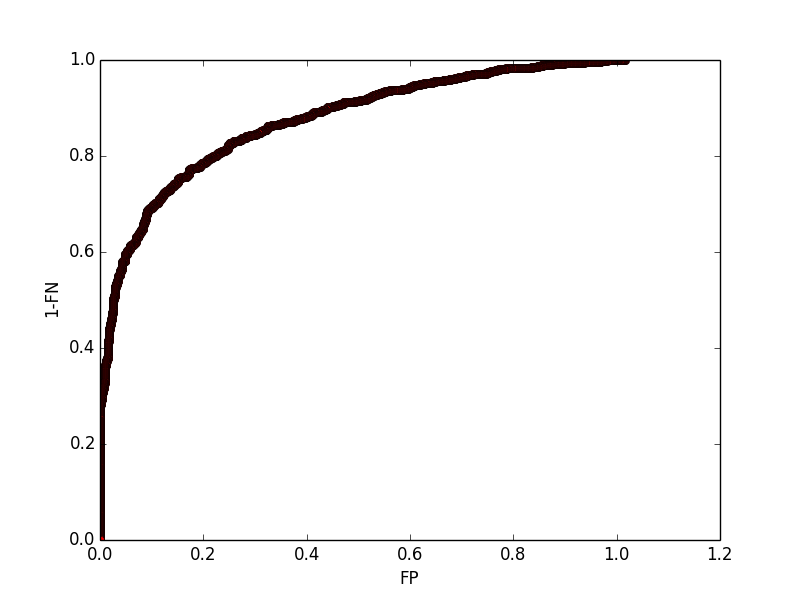
\includegraphics[scale=0.4]{../roc/outputs/scoresA.png}
                \caption{Curva ROC del sistema biométrico A}
                \label{fig:rocA}
        \end{subfigure}%
        \begin{subfigure}[b]{0.5\textwidth}
                \centering
                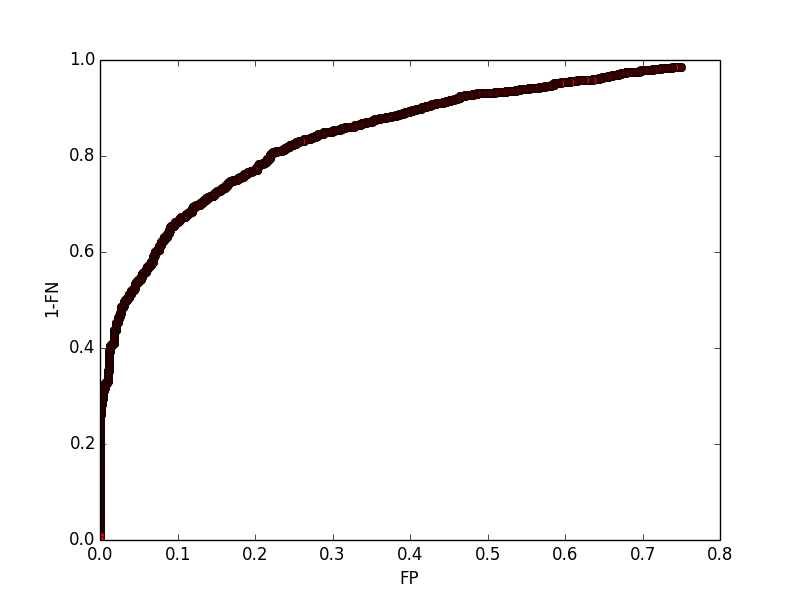
\includegraphics[scale=0.4]{../roc/outputs/scoresB.png}
                \caption{Curva ROC del sistema biométrico b}
                \label{fig:rocB}
        \end{subfigure}
    \caption{Curva ROC para dos sistemas biométricos}\label{fig:roc_curve}
\end{figure}
\newpage
\subsubsection{Obtener el valor FNR o el valor de FPR}
Uno de los datos que nos puede interesar para comparar dos sitemas biométricos o incluso para establecer el valor a partir del cual aceptamos o rechazamos, es que dado el valor del ratio de los falsos positivos obtener el valor del  ratio de los falsos negativos y el umbral para obtener este valor. Análogamente podemos querer el valor de los falsos postivos y el umbral dado un valor de falsos negativos.\par
Podemos ver un ejemplo de la ejecucición en el segmento de código \ref{roc:ratios}.\par

\begin{lstlisting}[language=python,label=roc:ratios,caption=Obtención de ratios y umbrales]

$ python roc_curve.py -c ../data/scores/scoresB_clientes.txt 
-i ../data/scores/scoresB_impostores.txt  -fp 0.6   
Dado el valor de fp: 0.6, el valor 
de fnr es: 0.0458041958042 y el umbral: 0.00434 

$ python roc_curve.py -c ../data/scores/scoresB_clientes.txt 
-i ../data/scores/scoresB_impostores.txt  -fn 0.3 -p
Dado el valor de fn: 0.3, el valor 
de fpr es: 0.129020979021 y el umbral: 0.079034 

\end{lstlisting}

Antes de continuar a la siguiente sección, aclaramos que los valores obtenidos en este apartado se obtienen si existen directamente de los datos y sino se interpolan a partir de la curva ROC.\par

\subsubsection{Obtener el área bajo la curva ROC}

El área bajo la curva ROC es una buena medida para evaluar numéricamente varios sistemas biométricos.\par
Hemos implementado esta medida mediante una aproximación a la integral de la curva y mediante la resolución de la integral mediante el método del trapecio. De los resultados que podemos ver en el segmento de código \ref{roc:aur}, vemos que tanto el área como los tiempos de ejecución varian en función del método empleado.\par
En la figura \ref{fig:aur}, vemos los resultados que hemos obenido.

\begin{lstlisting}[language=bash,label=roc:aur,caption=Calculo del área bajo la curva ROC para sistemas biométricos]
\$ python roc_curve.py -c ../data/scores/scoresB_clientes.txt 
-i ../data/scores/scoresB_impostores.txt  -a       
El área bajo la curva roc es igual a 0.624729082107 
(Coste temporal: 0.000113964080811)

\$ python roc_curve.py -c ../data/scores/scoresB_clientes.txt 
-i ../data/scores/scoresB_impostores.txt  -aA
El área bajo la curva roc es igual a 0.883082526448 
(Coste temporal : 5.70780491829)
\end{lstlisting}

\begin{figure}[ht]
    \centering
        \begin{subfigure}[b]{0.5\textwidth}
                \centering
                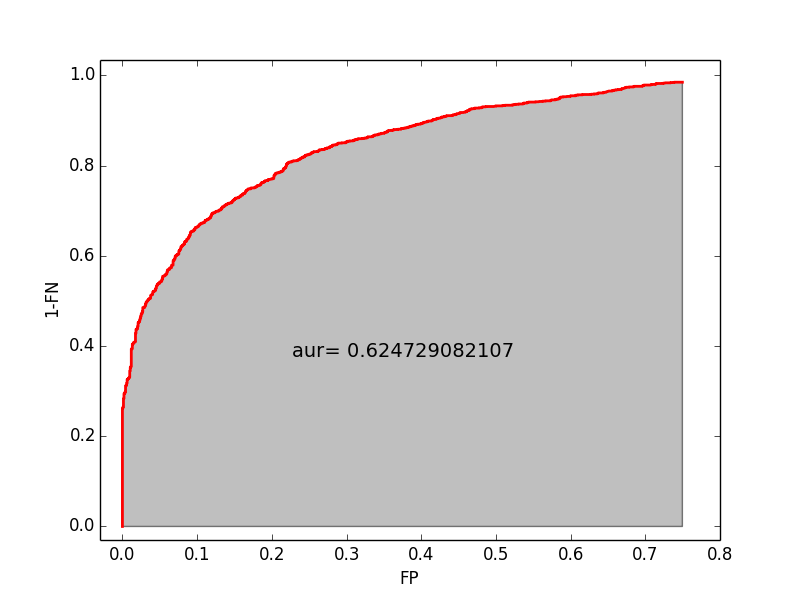
\includegraphics[scale=0.4]{../roc/outputs/aurB_metodo1.png}
                \caption{AUR método aproximado}
                \label{fig:aurAprox}
        \end{subfigure}%
        ~ 
        \begin{subfigure}[b]{0.5\textwidth}
                \centering
                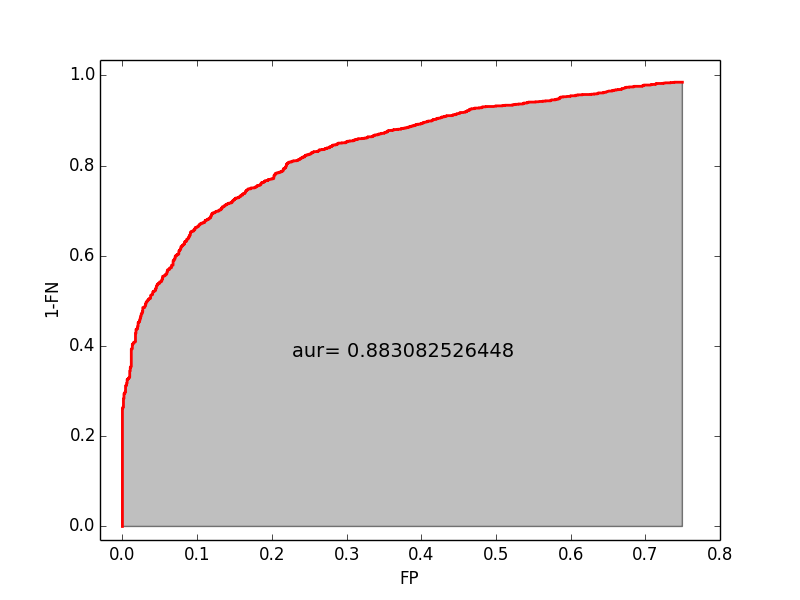
\includegraphics[scale=0.4]{../roc/outputs/aurB_metodo2.png}
                \caption{AUR método del trapecio}
                \label{fig:aurTrap}
        \end{subfigure}
    \caption{AUR}\label{fig:aur}
\end{figure}


\subsubsection{Obtener el factor d'}
Por útlimo calculamos el valor del factor d', que mide la discriminalidad de la técnica empleada. En el segmento de código \ref{roc:dprime} 

\begin{lstlisting}[language=python,label=roc:dprime,caption=Calculo del factor d-prime]
\$ python roc_curve.py -c ../data/scores/scoresB_clientes.txt 
-i ../data/scores/scoresB_impostores.txt  -d -s dprime
El factor dprime es 0.873481856448
\end{lstlisting}


\chapter{Implementación de PCA}
\section{PCA}
El siguiente ejercicio desarrollado es el análisis de las principales componentes de una imagen. Como entrada tenemos un conjunto de imágenes de caras de distintos sujetos y el número de dimeniones a las que queremos proyectar dichas imágenes.\par
Una vez leídas las imágenes y cargadas en memoria como un vector de número reales, reservamos un conjunto de imágenes para el anális de las principales componentes y otro conjuto para probar cómo funciona este análisis. En este caso hemos reservado un 50\% de las imágnes para el entrenamiento y el restante 50\% para las pruebas.\par
Para cada una de las imágenes calculamos su proyección en el nuevo espacio de componentes de dimensionalidad d'. En el ejemplo que hemos desarrollado 


\chapter{Schneiderman y Kanade}

\section{ Datos de entrada }

En primer lugar hemos preparado las imágenes para disponer de un conjunto de pruebas, otro para el desarrollo y un último para el test. El conjunto de entrenamiento lo empleamos para calcular las probabilidades que emplearemos en para la clasificación de una imagen en cara o no cara. El conjunto de desarrollo es un conjunto de imagenes distintas a las imágenes de entrenamiento empleadas para estimar el valor de $\lambda$. Finalmente tendremos un conjunto de test lo emplrearemos para calcular como funciona nuestro sistema.\par

Disponemos como parámetros de entrada de una serie de imágenes para el entreamiento expersadas mediante una serie de números de tipo flotante que corresponden con el valor del nivel de gris de la imagen normalizado. El primer paso que hemos desarrollado a consistido en leer estas imágenes y separar correctamente un porcentaje para entrenamiento y otro para test. El 80\% corresponderá al entrenamiento y el 20\% restante al test.\par

\section{Descripción del trabajo realizado}
\subsection {Entrenamiento}
Para cada una de las imágenes del test, las dividimos en regiones y cuatificamos estas regiones utilizando el algorimto c-medias con 100 iteraciones, seleccionamos 256 niveles, por lo tanto las regiones que en este punto son matrices de 5x5 se colapsan a un único valor. A partir de estos valores calculamos las probabilidades de que este valor que hemos cuantificado pertenezca a cara o no caras, es decir $P(q | caras)$ y $P(q | no cara)$, para esto hemos empleado vectores inicializaods a 0 y después normalizados, pero como el conjunto de entrenamiento que estabamos empleando era muy disperso hemos realizado un suavizado de Laplace. También deberemos calcular la probabilidad de que en una posición de la imagen dado un valor cuantificado y si es cara o no cara, es decir  $P(pos|q, caras)$ y $P(pos|q, no cara)$. Todas estas probabilidades nos las devolverá la función train que vemos en el segmento de código \ref{sk:train}, así como el tamaño de la ventana entrenado. 

\begin{lstlisting}[language=python,label=roc:rocdata,caption=EDA con la que gestionar la curva ROC]
def train(faces, not_faces, num_regions, q_levels):
	...
    return p_q_faces, p_q_notFaces, p_pos_q_faces, 
    	   p_pos_q_notFaces, width
\end{lstlisting}


\subsection{Ajuste del parámetro $\lambda$}

Una vez tenemos las probabilidades entrenadas utilizaremos el conjunto de test y calcularemos la probabilidad de que sea cara o no cara utilizando la regla de decisión descrita por Schneiderman y Kanade e imprimimos la media de las probabilidades de que la imagen sea cara y la media de las probabilidades de que la imagen no sea cara. Podemos ver un ejemplo de como ejecutar el algoritmo en modo desarrrollo en el segmento de código \ref{sk:dev}.\par

\begin{lstlisting}[language=bash,label=sk:dev,caption=Ejecución en modo desarrollo]
$ python sk.py -f ../data/caras/dev_faces400 
               -n ../data/caras/dev_notFaces400 -d 
\end{lstlisting}

Estas medias las escribiremos en un fichero de texto plano, \textit{test} y mediante otro pequeño programa en python, \textit{lamda.py}, dónde leemos las probabilidades medias que hemos obtenido para caras y no caras y establecemos como lamda un valor que se encuentre en un punto medio entre la probabilidad de que  la imagen sea cara y que sea no cara. Claramente este valor se verá muy afectado por datos anómalos ya que influyen mucho en la media.\par

\subsection{Prueba del sistema}

Una vez determinado el valor de lambda probaremos como funciona el sistema que hemos entrenado con datos de prueba. Para esto cogemos un nuevo conjunto de datos que no hayamos empleado para entrenar el sistema y calcularemos los veredaderos y falsos positivos así como los verdaderos y falsos negativos. Para ejecutar el sistema en modo de prueba deberíamos lanzar una orden como la que vemos el segmento de código \ref{sk:test}.

\begin{lstlisting}[language=bash,label=sk:test,caption=Ejecución en modo pruebas]
$ python sk.py -f ../data/caras/dev_faces2000 
                -n ../data/caras/dev_notFaces2000 
                -l 0.090909091113 -d 
                -ft ../data/caras/faces_test600 
                -nt ../data/caras/notfaces_test600 -t-f
\end{lstlisting}

Ejecutaríamos este análisis del sistama con distintos conjuntos de prueba y obtendríamos una medida de la robustez del sistema. Sin embargo, como el conjunto de test y de prueba que hemos empleado pertenecen a una misma base de datos de imagenes el sistema se comporta demasiado favorablemente, esta sobreentrenado. Esto lo comprobamos al probar nuestro sistema de reconocimiento con una imagen distinta. Los restultados pueden encontrarse en el fichero de texto plano \textit{test\_error}

\subsubsection{Uso del reconocedor}
La útlima fase consiste en con el reconocedor entrenado buscar las caras dentro de una imagen.\par
Leemos y cargamos la imagen en memoria, cogemos secciones del tamaño de la ventana que hemos entrenado ya al igual que en la fase de pruebas calculamos la probabilidad de que en una region dada haya una cara si es mayor al lambda que hemos establecido en la fase de test. \par

Nos ha quedado pendiente desarrollar el dibujado de las regiones dónde ha encontrado cara, así como reducir el tamaño de la imagen para que las caras que encontremos sean invariantes al tamaño como explican Schneiderman y Kanade en su algoritmo.\par

La ejecución  se realiza como vemos en el segmento de código \ref{sk:reconocimiento}
\begin{lstlisting}[language=bash,label=sk:reconocimiento,caption=Ejecución en modo reconocedor]
\$ python sk.py -f ../data/caras/dev_faces2000 
                -n ../data/caras/dev_notFaces2000
                -l 0.090909091113 -t -i ../data/caras/jr.png
\end{lstlisting}


\chapter{Fusión de scores}
Cuanto disponemos de varios resultados obtenidos de distintas fuentes biométricas para poder evaluar como afectan cada uno de los resultados en la decisión desarrollaremos un sistema de fusión de caracterísicas biométricas.

\section{Datos de entrada}
Para este ejercicio disponemos de ficheros con texto plano cuya última columna nos indica si el dato es un cliente o un impostor y en las columnas anteriores tenemos los resultados de los distintos sistemas biométricos. En este caso únicamente 2 scores.

\section{Desarrollo realizado}
\subsection{Tratamiento de los datos de entrada}
En primer lugar desarrollamos un pequeño script bash, que separe los scores de los clientes y de los impostores y se quede con una subsección de los mismos, para acelerar los cálculos. En caso de llevar este sistema a producción el número de elementos en el subconjunto deberá se el total de los elementos disponibles.\par

\subsection{Fusión de scores}
Con los datos ya preparados realizamos un script en python que lea estos datos y calcule el peso para cada score de modo que se minimice el área bajo la curva ROC.\par
En el listado de código \ref{fusion:sol} podemos ver las opciones para lanzar el script.\par


\begin{lstlisting}[language=python,label=fusion:uso, caption=PCA cuado n es menor d]

$ python fusion.py --help                         
usage: fusion.py [-h] [-tr TR] [-te TE] [-p]

Fuse some scores
optional arguments:
  -h, --help          show this help message and exit
  -tr TR, --train TR  Scores for train data
  -te TE, --test TE   Scores for test data
  -p, --plot          Make plot
\end{lstlisting}


\section{Resultados}

A continuación, en el segmento de código \ref{fusion:sol}, vemos los resultados de la fusión de los dos scores de modo que minimicen el área bajo la curva ROC. Y en la figura \ref{fig:fusion} vemos como se distribuyen los dos scores tanto en entrenamiento como en pruebas.\par

\begin{lstlisting}[language=python,label=fusion:sol, caption=PCA cuado n es menor d]
$ python fusion.py -tr ../data/fusion/train_small -te ../data/fusion/test_small -p
El valor máximo del área bajo la curva ROC= 1.423700 
Con los pesos:
  [ 0.60, 0.40 ]
\end{lstlisting}

\begin{figure}[h!]
  \centering
      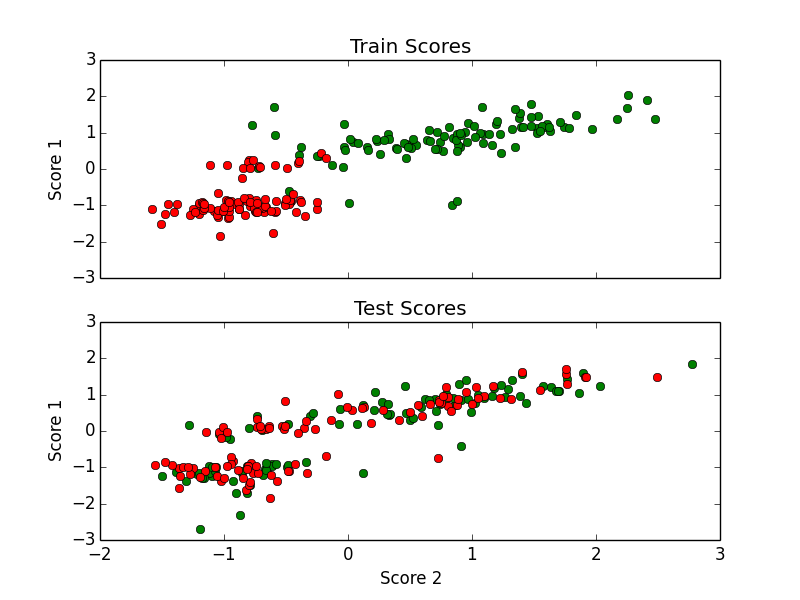
\includegraphics[width=0.7\textwidth]{../fusion/fusion.png}
  \caption{ Scores en train y en test}
  \label{fig:fusion}
\end{figure} 




\end{document}